\section{Gewöhnliche Differentialgleichungen (DGL)}

Kurz \textcolor{blue}{DGL}, die Veränderung ($y'(x)$) einer Funktion an einem Punkt ist abhängig vom Wert
der Funktion selbst
$$\frac{dy}{dx} = f(x, y(x))$$

Eine solche gleichung nennt man gewöhnliche Differentialgleichung 1. Ordnung
(1. Ordnung weil nur die erste Ableitung vorkommt, engl. ODE = Ordinary
Differential Equation)



\subsection{gewöhnliche Differentialgleichung $n$-ter Ordnung}

Eine Gleichung in der Ableitungen einer unbekannten Funktion $y = y(x)$ bis zur $n$-ten
Ordnung auftreten.

Explizite Form:
{\Large
$$y^{(n)}(x) = f(x, y(x), y'(x), ..., y^{(n-1)}(x))$$
}

Beispiel:
$$y''(x) = y'(x)^3 * y(x) + cos(x) = f(x, y(x), y'(x))$$

Gesucht sind Lösungen $y : [a,b] \to \R = y(x)$ dieser Gleichung wobei die Lösungen
$y$ auf einem Interval $[a,b]$ definiert sind.



\subsection{Anfangswertproblem (AWP)}

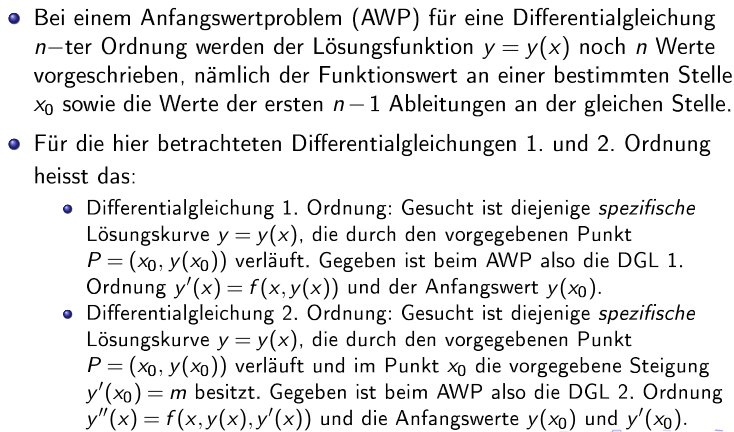
\includegraphics[scale=0.32]{diff-awp}












\subsection{Richtungsfelder (1. Ordnung)}

Die verschiedenen Lösungen einer DGL 1. Ordnung lassen sich als Richtungsfeld
darstellen. Hierbei wird in jedem Punkt $(x,y(x))$ die Steigung $y'(x) = f(x, y(x))$
als Pfeil eingezeichnet.

In dem man diesen Pfeilen entlang einer Kurve ''folgt'' hat man eine
spezifische Lösung.






\section{Einzelschrittverfahren}

\begin{itemize}
	\item gesucht: Funktion $y : [a, b] \to \R$
	\item Anfangsbediung $y(a) = y_0$
	\item Schrittweite $h = \frac{b-a}{n}$ wählen und Intervall $[a,b]$
	      mit $n+1$ Gittsterstellen $x_i = a + i*h \; | \; i = 0,1,...,n$
	      aufteilen
	\item Ziel: für alle Gitterstellen $x_i$ die Näherungen $y_i$ bestimmen
	\item im Einzelschrittverfahren wird die nächste stelle $x_{i+1}$ Anhand
	      der bekannten Lösung für $x_i \; | \; (x_0 = a, y(x_0) = y_0)$ berechnet
	      \begin{align*}
		      x_{i+1} & = x_i + h                     \\
		      y_{i+1} & = y_i + \mathrm{Steigung} * h
	      \end{align*}

	      Mit der Steigung als eine numerische Näherung für
	      $y'(x) \; | \; x \in [x_i, x_{i+1}]$
	\item Die verschiedenen Einzelschrittverfahren unterscheiden sich nur
	      in der Bestimmung der Steigung
\end{itemize}



\subsection{Euler-Verfahren}
% TODO code


\subsubsection{klassisches Euler-Verfahren}

Gegeben Anfangswertproblem:
$$\frac{dy}{dx} = f(x, y(x)) \quad \mathrm{mit} \; y(a) = y_0$$


\begingroup
\addtolength{\jot}{0.5em}
\large

Algorithmus:

\begin{multicols}{2}
	Für $i = 0,1,..,n-1$:
	\begin{align*}
		x_{i+1} & = x_i + h       \\
		k_1     & = f(x_i, y_i)   \\
		y_{i+1} & = y_i + h * k_1
	\end{align*}

	\columnbreak

	Wobei:
	\begin{align*}
		x_0 & = a       \\
		x_i & = a + i*h \\
		h   & = (b-a)/n
	\end{align*}
	\vspace{\fill}
\end{multicols}
\endgroup


\subsubsection{Mittelpunkt Euler-Verfahren}

Anstatt das wie beim klassischen direkt die Steigung am Punkt zu $x_i, y_i$ nehmen
wird die Steigung im Mittelpunkt $x_i + h/2$ verwendet.


\begingroup
\addtolength{\jot}{0.5em}
\large
Algorithmus:

Für $i = 0,1,..,n-1$:
\begin{align*}
	x_{h/2} & = x_i + h/2                        \\
	k_1     & = f(x_i, y_i)                      \\
	k_2     & = f(x_i + h/2, \; y_i + h/2 * k_1) \\
	x_{i+1} & = x_i + h                          \\
	y_{i+1} & = y_i + h * k_2
\end{align*}
\endgroup


\subsubsection{modifiziertes Euler-Verfahren}

Unterschied hier ist das der Durchschnitt der Steigungen an $x_i$ und $x_{i+1}$
verwendet wird.

\begingroup
\addtolength{\jot}{0.5em}
\large
Algorithmus:

Für $i = 0,1,..,n-1$:
\begin{align*}
	k_1     & = f(x_i, y_i)                                \\
	k_2     & = f(x_i + h, \; y_i + h * k_1)               \\
	x_{i+1} & = x_i + h                                    \\
	y_{i+1} & = y_i + \frac{h}{2} k_1 + \frac{h}{2} k_1    \\
	        & = y_i + h * \left(\frac{k_1 + k_2}{2}\right)
\end{align*}
\endgroup



\subsection{Fehlerordnung}

Bemerkungen:
\begin{itemize}
	\item bei unseren Verfahren ist Konsistenzordnung = Konvergenzordnung
	\item durch Verkleinern von $h$ kann der Fehler theoretisch beliebig klein
	      werden aber dann überwiegen Rundungsfehler
	\item das klassiche Euler-Verfahren hat $p=1$, Mittelpunkt \& modifiziertes
	      $p=2$
	\item vierstufiges Runge-Kutta hat $p=4$
\end{itemize}

\subsubsection{lokaler Fehler/Konsistenzordnung}

Gegeben:
\begin{itemize}
	\item DGL $y'(x) = f(x, y(x))$ mit Anfangsbediung $y(x_i) = y_i$
	\item Exakte Lösung $y(x)$
	\item Näherungswert $y_{i+1}$ für $y(x_{i+1})$ aus numerischem
	      Verfahren mit Schrittweite $h$
\end{itemize}


Der \textcolor{cyan}{lokale Fehler nach einer Iteration} ist dann definiert als:
$$\varphi(x_i, h) = y(x_{i+1}) - y_{i+1}$$

\begingroup
Ein numerisches Verfahren hat \textcolor{cyan}{Konsistenzordnung $p$} falls:
\large
\begin{multicols}{2}
	$$|\varphi(x_i, h)| \le C * h^{p+1}
		\vspace{\fill}
	$$
	\columnbreak
	\begin{itemize}
		\item für genügend kleine Schrittweite $h$
		\item Konstante $C > 0$ hängt von DGL ab
		\item \textcolor{cyan}{wird $h$ halbiert, geht der lokale Fehler
			      um Faktor $(\frac{1}{2})^{p+1}$ runter}
	\end{itemize}
\end{multicols}
\endgroup

Da $C$ konstant $\rarr$ Fehler ist rein von gewählter Schrittweite abhängig
und nimmt mit $h^{p+1}$ rasant ab für Verfahren mit
\textcolor{orange}{hoher Fehlerordnung (GUT)}


\subsubsection{globaler Fehler/Konvergenzordnung}


Gegeben:
\begin{itemize}
	\item DGL $y'(x) = f(x, y(x))$ mit Anfangsbediung $y(x_i) = y_i$
	\item Exakte Lösung $y(x)$
	\item Näherungswert $y_n$ für $y(x_n=x_0 + n h)$ aus numerischem
	      Verfahren mit Schrittweite $h$
\end{itemize}

Der \textcolor{cyan}{globale Fehler nach $n$ Iterationen} ist dann definiert als:
$$\varphi(x_i, h) = y(x_n) - y_n$$

Ein Verfahren hat \textcolor{cyan}{Konvergenzordnung $p$} falls:
$$|y(x_n) - y_n| \le C * h^p$$










\subsection{Runge-Kutta Verfahren}

Wie Euler-Verfahren aber nochmehr $k_i$ Zwischenpunkte für die Steigung.

Gegeben Anfangswertproblem:
$$\frac{dy}{dx} = f(x, y(x)) \quad \mathrm{mit} \; y(a) = y_0$$


\subsubsection{klassisches vierstufiges Runge-Kutta Verfahren}


\begingroup
\addtolength{\jot}{0.5em}
\large
Für $i = 0,1,..,n-1$:
\begin{align*}
	x_{h/2} & = x_i + h/2                                       \\
	k_1     & = f(x_i, y_i)                                     \\
	k_2     & = f(x_i + h/2, \; y_i + h/2 * k_1)                \\
	k_3     & = f(x_i + h/2, \; y_i + h/2 * k_2)                \\
	k_4     & = f(x_i + h, \; y_i + h * k_3)                    \\
	x_{i+1} & = x_i + h                                         \\
	y_{i+1} & = y_i + h * \frac{1}{6}(k_1 + 2k_2 + * 2k_3 + k4)
\end{align*}
\endgroup


\subsubsection{allgemeines s-stufiges Runge-Kutta Verfahren}


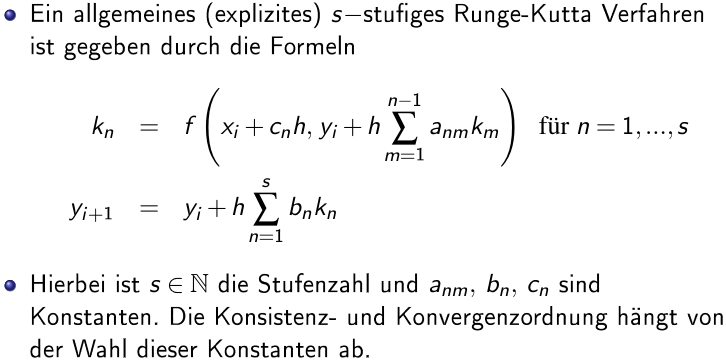
\includegraphics[scale=0.33]{diff-runge-kutta-allg-algo}

Die Koeffizienten können wie folgt in einer Matrix notiert werden

\begin{center}
	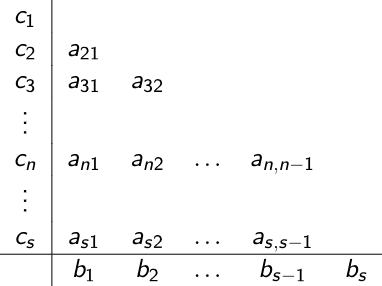
\includegraphics[scale=0.33]{diff-runge-kutta-allg-koeff}
\end{center}


Die Euler-Verfahren können auch so dargestellt werden

\begin{minipage}{0.35\linewidth}
	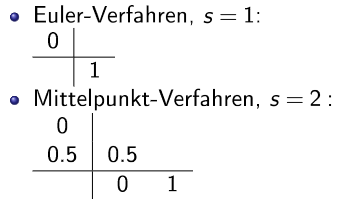
\includegraphics[scale=0.33]{diff-runge-kutta-koeff-bsp-1}
\end{minipage}
\hfill
\begin{minipage}{0.55\linewidth}
	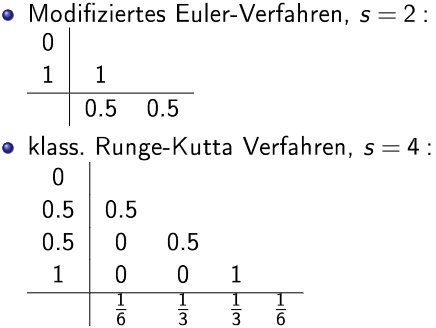
\includegraphics[scale=0.33]{diff-runge-kutta-koeff-bsp-2}
\end{minipage}




\subsection{Systeme von Differentialgleichungen}

DGL von k-ter Ordnung auf ein System von DGL 1. Ordnung
zurückführen.


Anhand Beispiel: (8.9 im Skript)

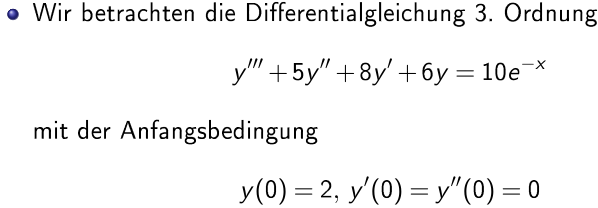
\includegraphics[scale=0.33]{diff-systeme-bsp-1}\\
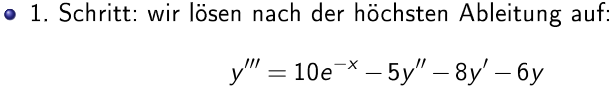
\includegraphics[scale=0.33]{diff-systeme-bsp-2}\\
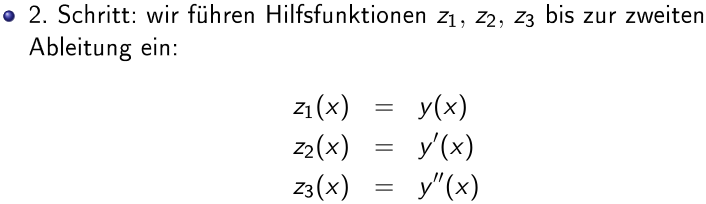
\includegraphics[scale=0.33]{diff-systeme-bsp-3}\\
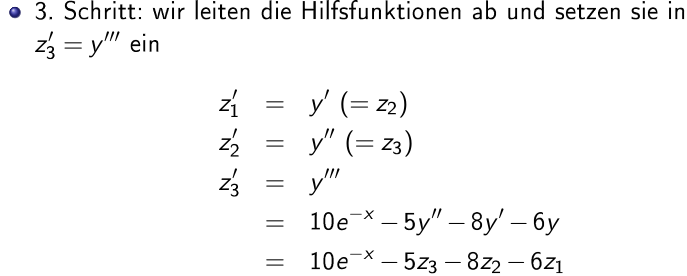
\includegraphics[scale=0.33]{diff-systeme-bsp-4}\\
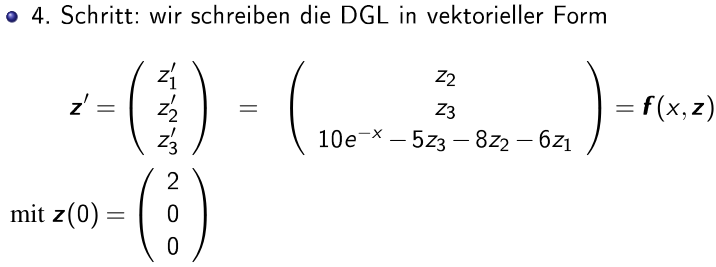
\includegraphics[scale=0.33]{diff-systeme-bsp-5}

\begingroup
\large

$$ \v f(x, \v z) =
	\begin{pmatrix}
		0  & 1  & 0  \\
		0  & 0  & 1  \\
		-5 & -8 & -6
	\end{pmatrix} \v z
	+ \begin{pmatrix} 0 \\ 0 \\ 10e^{-x} \end{pmatrix}
$$


So wurde aus einer DGL 3. Ordnung $\rarr$ drei DGL 1. Ordnung mit folgendem
Anfangswertproblem 1. Ordnung
$$\v{z'} = \v f(x, \v z) \; \mathrm{mit} \; \v z(0) =
	\begin{pmatrix} y(0) \\ y'(0) \\ y''(0) \end{pmatrix}
$$
\endgroup



\subsubsection{Lösen eines DGL Systemes}

Identisch zu bekannten Runge-Kutta verfahren, einfach alles Vektoren.
(Hochgestellter Index in Klammern wieder für Iterationen weil tiefe für
einzelne Vektorelemente)


Beispiel Euler: für $i = 0,1,..,n-1$:
\begin{align*}
	x_{i+1}          & = x_i + h                     \\
	\v k_1           & = \v f(x_i, \iter{\v y}{i})   \\
	\iter{\v y}{i+1} & = \iter{\v y}{i} + h * \v k_1
\end{align*}


mit:
\begin{multicols}{2}
	$$\v y(x) = \begin{pmatrix} y_1(x) \\ \vdots \\ y_k(x) \end{pmatrix}$$
	$$\v{y'}(x) = \begin{pmatrix} y'_1(x) \\ \vdots \\ y'_k(x) \end{pmatrix}$$

	\columnbreak

	$$\v f(x, \v y(x)) = \begin{pmatrix} f_1(x, \v y(x)) \\ \vdots \\ f_1(x, \v y(x)) \end{pmatrix}$$
\end{multicols}

